%!TEX root =  ../Report.tex

\section{Part 2: The Effects of Ties}                               
\label{sec: Part 2}

In previous sections, it was mentioned that $A^*$ \emph{search} is an informed search algorithm, and therefore uses an evaluation function, denoted as $f(n) = g(n) + h(n)$. In this function, $g(n)$ is the traveled distance from node $n$ to the initial state, and $h(n)$ is the heuristic function. In our priority queue, we will be prioritizing nodes with the smallest $f(n)$ value, but the problem is that multiple nodes can have the same $f(n)$ value. So what do we do if the smallest $f(n)$ value happens to be in a tie with 1 or more other nodes? 


We will look at the run times for breaking this tie by prioritizing the nodes with the superior $g(n)$ value. In particular, we will implement this through our \texttt{Node} class, by using this line for prioritizing nodes with a larger $g(n)$:
\begin{lstlisting}
    return self.g >= otherNode.g #tie breaker for larger g value
\end{lstlisting}

and changing this line to the following for prioritizing smaller $g(n)$ values:

\begin{lstlisting}
    return self.g < otherNode.g #tie breaker for smaller g value
\end{lstlisting}

The way this works is that the \texttt{heapq} library makes comparisons for each item it has by using the \texttt{<} operator. When two $f(n)$ values are the same, we defined this in our \texttt{Node} class and it will go to the line above and choose either the node with the larger or smaller $g(n)$ value. Below are the results.

\begin{figure}[H]
  \centering
  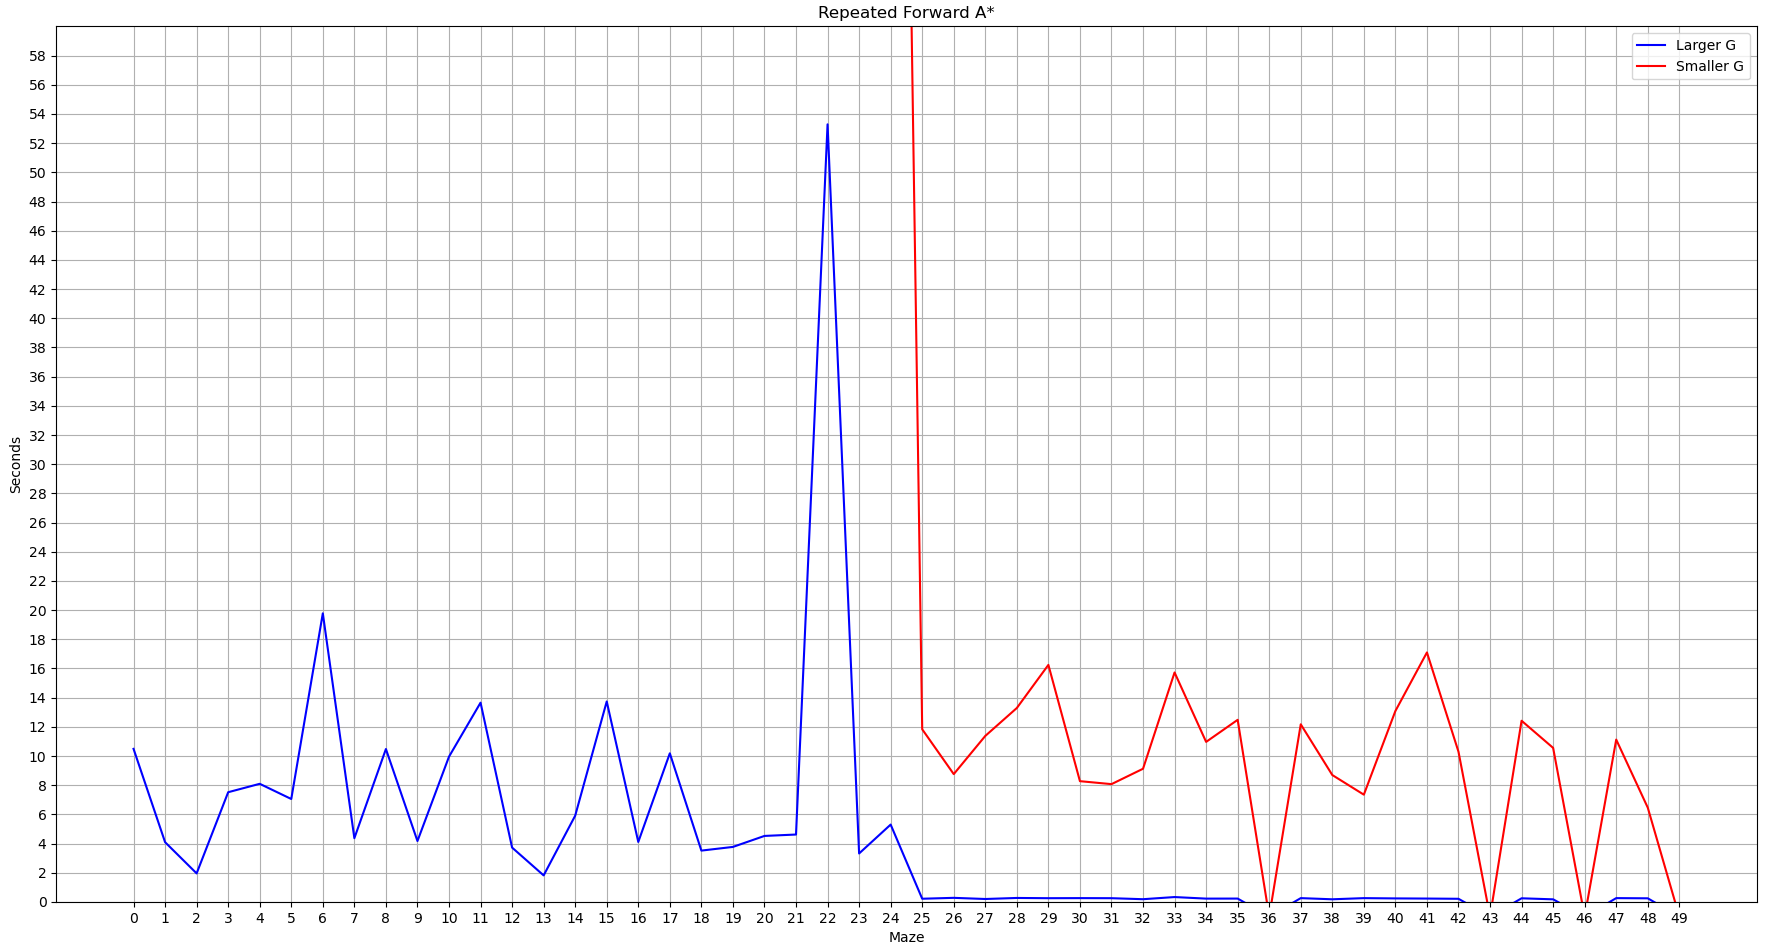
\includegraphics[width=1\linewidth]{Report/Part2/Figure_1.png}  
\caption{Repeated Forward $A^*$ $f(n)$ tie-breaker comparison}
\end{figure}

In the test, mazes 0-24 were the backtracked mazes and mazes 25-49 were the random mazes. It can be seen that choosing the smaller $g(n)$ value results in considerably longer run times, to the point where in our backtracked mazes it was taking upwards of 200 seconds (outside the range of this graph). It is also important to note that for mazes where the run time is at 0, it is because the solution was not found. This means either the start or goal node was blocked off by walls.


Our results show that using a larger $g(n)$ value as the tie breaker performs significantly better than using a smaller $g(n)$ value, and we will now explore the reason for this. 


Lets assume we run $A^*$ \emph{search} on the graph below, where $A1$ is our start and $E5$ is our goal. Heuristic values are shown in each cell.

\begin{figure}[H]
  \centering
  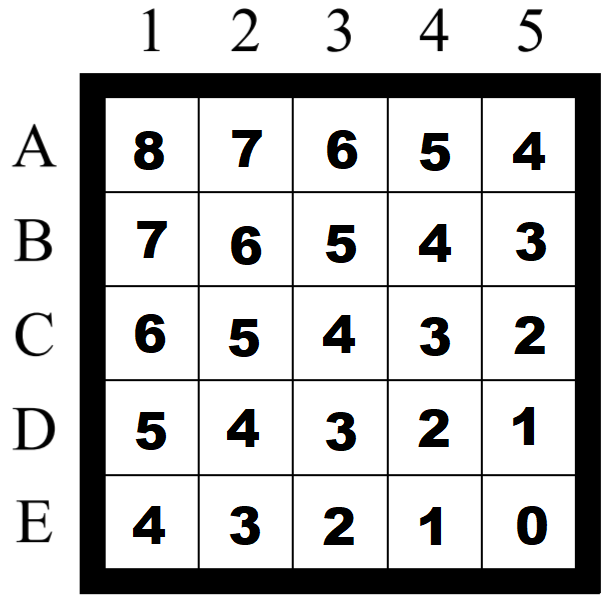
\includegraphics[width=0.31\linewidth]{Report/Part2/g tie breaker/samplegraph.png}  
\caption{Sample maze}
\end{figure}

We will first begin with an $A^*$ \emph{search} where the larger $g(n)$ is favored.
\linebreak
\begin{figure}[H]
\begin{subfigure}[b]{.3\textwidth}
  \centering
  \includegraphics[width=0.95\linewidth]{Report/Part2/g tie breaker/larger g/1.png}  
\end{subfigure}
\begin{subfigure}[b]{.3\textwidth}
  \centering
  \includegraphics[width=0.95\linewidth]{Report/Part2/g tie breaker/larger g/2.png}  
\end{subfigure}
\begin{subfigure}[b]{.3\textwidth}
  \centering
  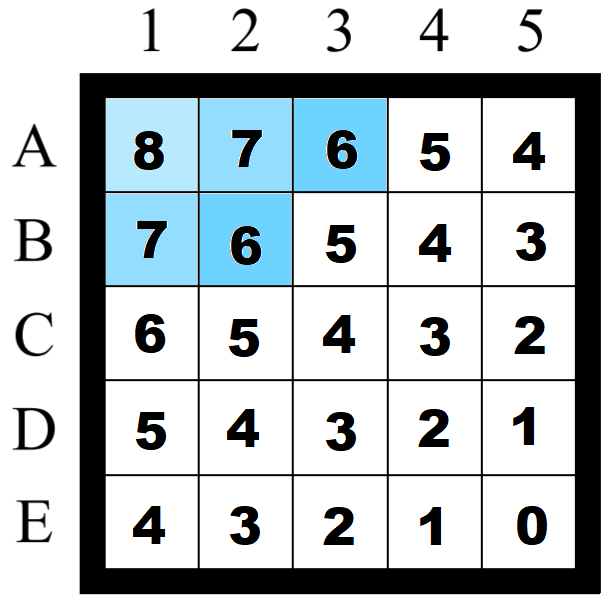
\includegraphics[width=0.95\linewidth]{Report/Part2/g tie breaker/larger g/3.png}  
\end{subfigure}
\newline
\linebreak
\begin{subfigure}[b]{.3\textwidth}
  \centering
  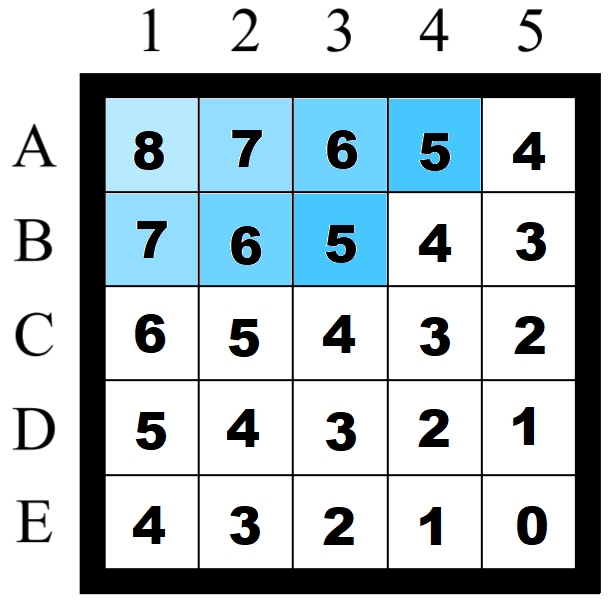
\includegraphics[width=0.95\linewidth]{Report/Part2/g tie breaker/larger g/4.png}  
\end{subfigure}
\begin{subfigure}[b]{.3\textwidth}
  \centering
  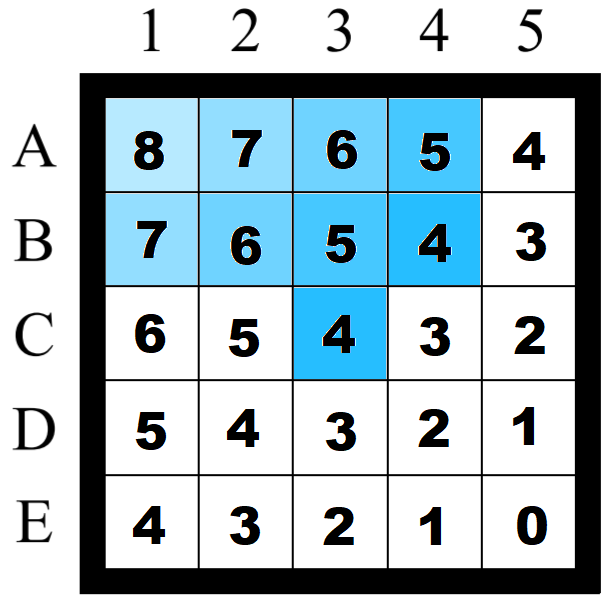
\includegraphics[width=0.95\linewidth]{Report/Part2/g tie breaker/larger g/5.png}  
\end{subfigure}
\begin{subfigure}[b]{.3\textwidth}
  \centering
  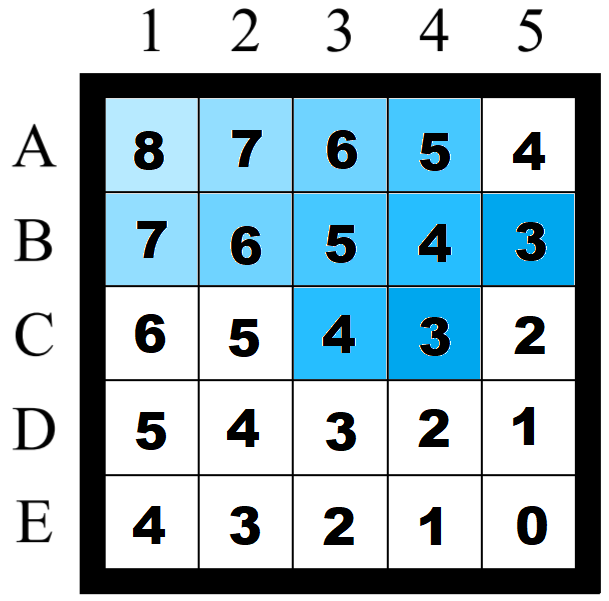
\includegraphics[width=0.95\linewidth]{Report/Part2/g tie breaker/larger g/6.png}  
\end{subfigure}
\newline
\linebreak
\begin{subfigure}[b]{.3\textwidth}
  \centering
  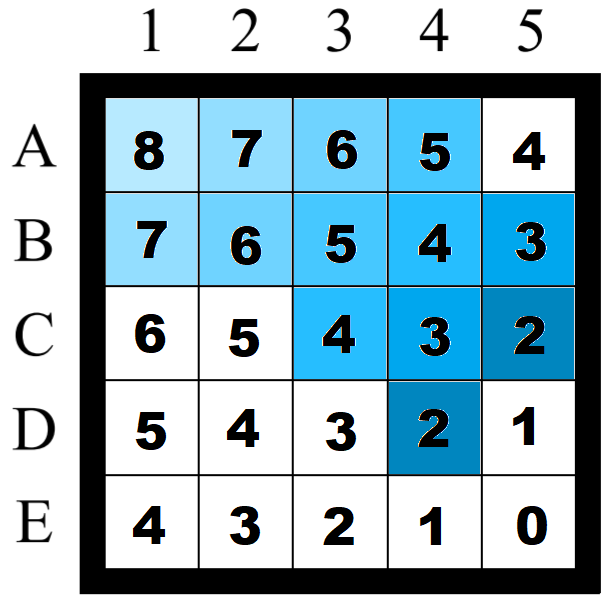
\includegraphics[width=0.95\linewidth]{Report/Part2/g tie breaker/larger g/7.png}  
\end{subfigure}
\begin{subfigure}[b]{.3\textwidth}
  \centering
  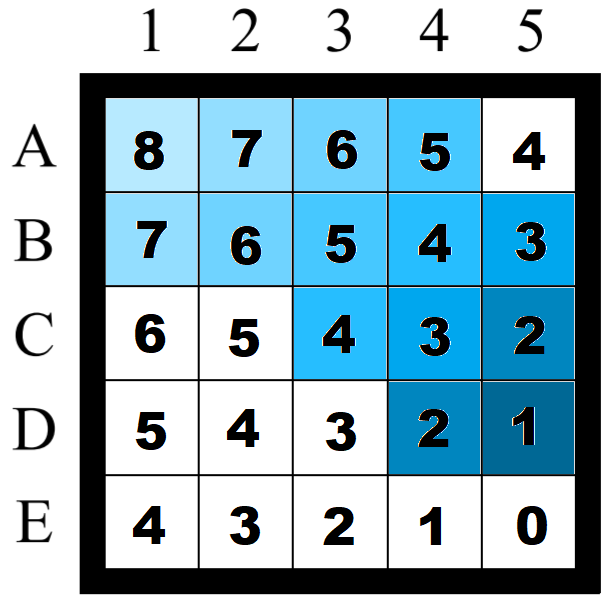
\includegraphics[width=0.95\linewidth]{Report/Part2/g tie breaker/larger g/8.png}  
\end{subfigure}
\begin{subfigure}[b]{.3\textwidth}
  \centering
  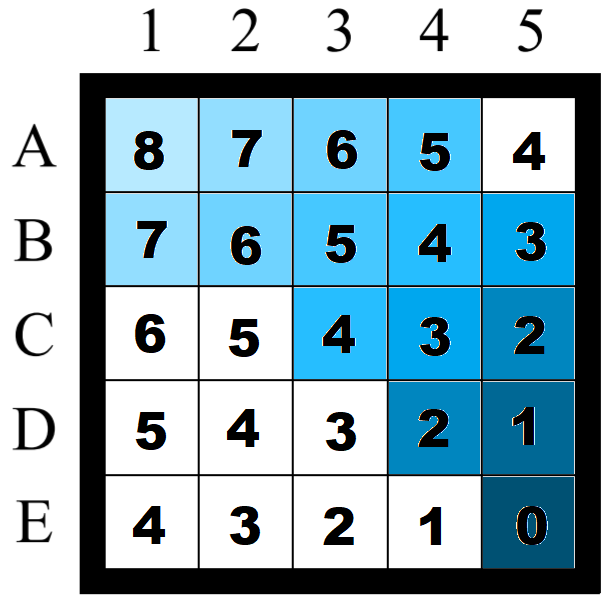
\includegraphics[width=0.95\linewidth]{Report/Part2/g tie breaker/larger g/9.png}  
\end{subfigure}


\caption{Forward $A*$ larger $g(n)$}
\end{figure}

As we observe, the solution is found in iteration 9 of the search. For each node expanded, the $f(n)$ value is actually always the same, since no obstacles exist and each step has a cost of 1. Therefore, we expand the nodes with the largest distance from the start node, since those have the largest $g(n)$ values.


Now lets look at the run through of {Forward $A^*$} which prioritizes a smaller $g(n)$.
\linebreak
\begin{figure}[H]
\begin{subfigure}[b]{.3\textwidth}
  \centering
  \includegraphics[width=0.95\linewidth]{Report/Part2/g tie breaker/smaller g/1.png}  
\end{subfigure}
\begin{subfigure}[b]{.3\textwidth}
  \centering
  \includegraphics[width=0.95\linewidth]{Report/Part2/g tie breaker/smaller g/2.png}  
\end{subfigure}
\begin{subfigure}[b]{.3\textwidth}
  \centering
  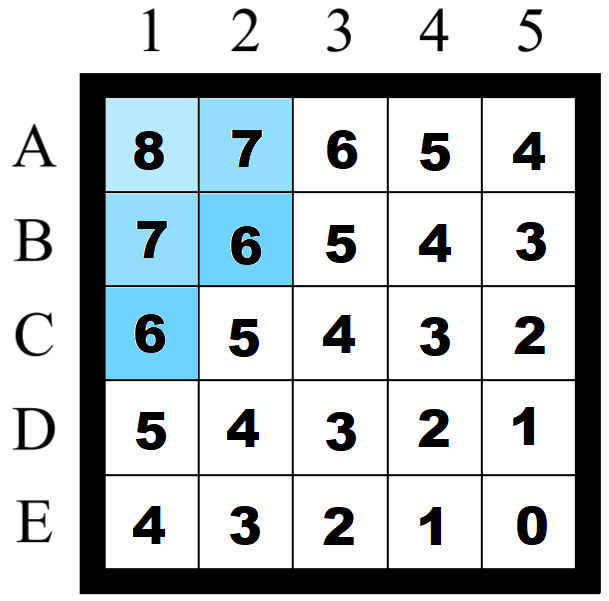
\includegraphics[width=0.95\linewidth]{Report/Part2/g tie breaker/smaller g/3.png}  
\end{subfigure}
\newline
\linebreak
\begin{subfigure}[b]{.3\textwidth}
  \centering
  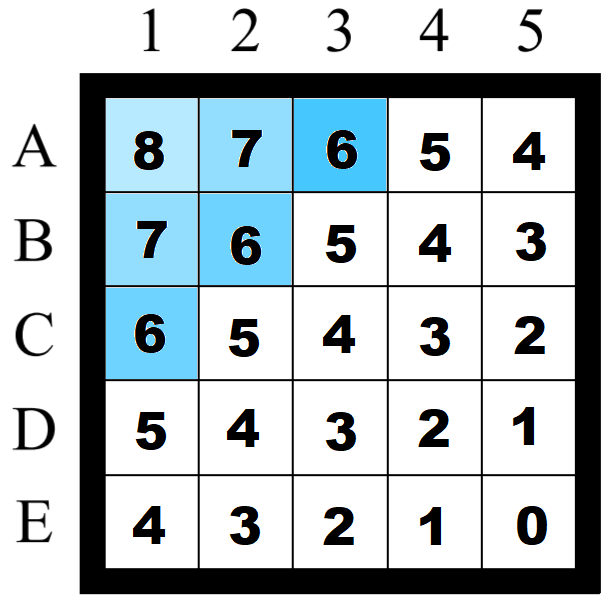
\includegraphics[width=0.95\linewidth]{Report/Part2/g tie breaker/smaller g/4.png}  
\end{subfigure}
\begin{subfigure}[b]{.3\textwidth}
  \centering
  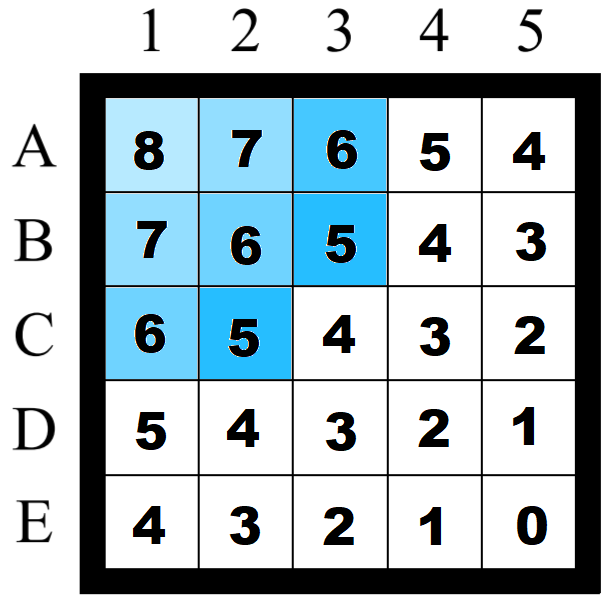
\includegraphics[width=0.95\linewidth]{Report/Part2/g tie breaker/smaller g/5.png}  
\end{subfigure}
\begin{subfigure}[b]{.3\textwidth}
  \centering
  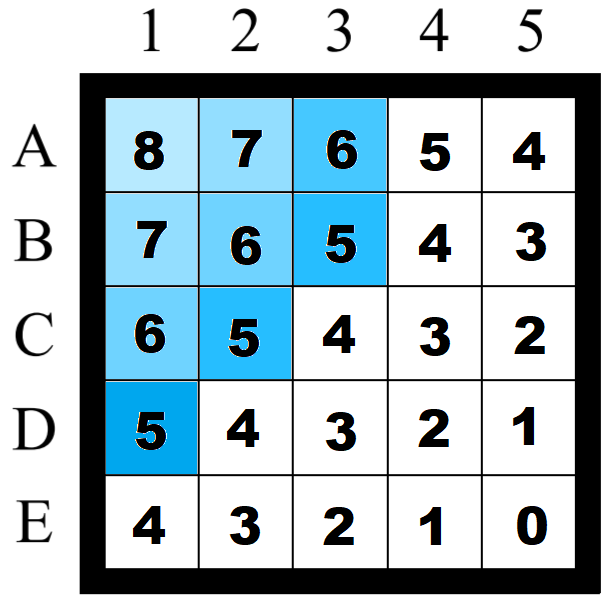
\includegraphics[width=0.95\linewidth]{Report/Part2/g tie breaker/smaller g/6.png}  
\end{subfigure}
\newline
\linebreak
\begin{subfigure}[b]{.3\textwidth}
  \centering
  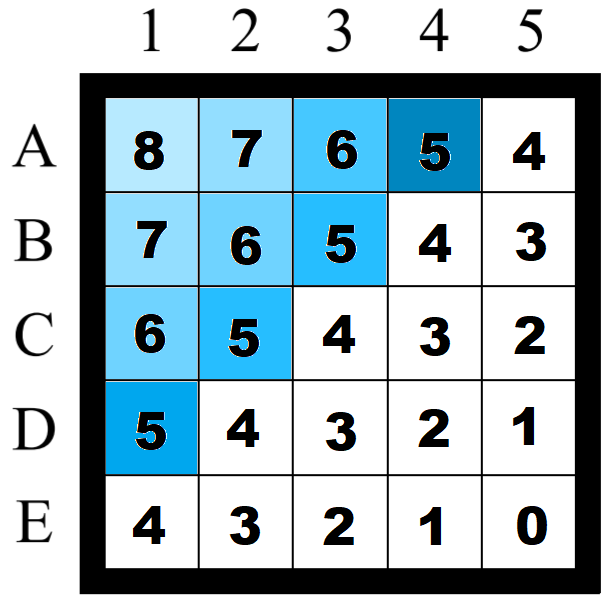
\includegraphics[width=0.95\linewidth]{Report/Part2/g tie breaker/smaller g/7.png}  
\end{subfigure}
\begin{subfigure}[b]{.3\textwidth}
  \centering
  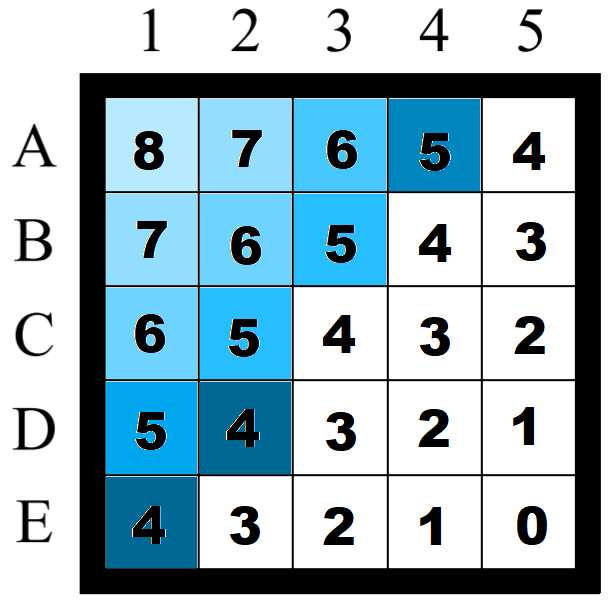
\includegraphics[width=0.95\linewidth]{Report/Part2/g tie breaker/smaller g/8.png}  
\end{subfigure}
\begin{subfigure}[b]{.3\textwidth}
  \centering
  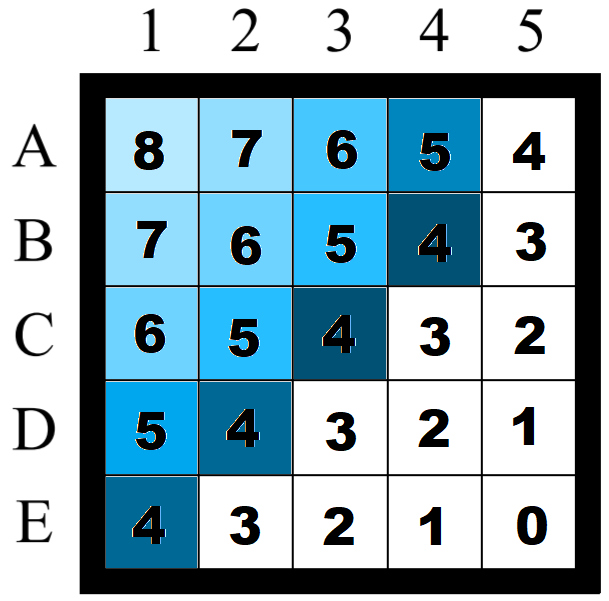
\includegraphics[width=0.95\linewidth]{Report/Part2/g tie breaker/smaller g/9.png}  
\end{subfigure}


\caption{Forward $A*$ smaller $g(n)$}
\end{figure}

In the results we see that by iteration 9, we have not reached the goal. In fact, it only seems that half of the map has been explored. So why is this the case? Logically, this is because each node inherently has the same $f(n)$ value, once again, because of there being no obstacles, and the cost of each step being 1. Therefore, the priority is on the nodes closest to the start.


But there is a deeper meaning behind choosing the larger or smaller $g(n)$ value in this situation. If we re-examine the above to tests, we notice something. It is that for the iterations where the larger $g(n)$ value is favored, $A^*$ \emph{search} acts the same as \emph{Depth First Search}. And on the other-hand, for the iterations where the smaller $g(n)$ value is favored, $A^*$ \emph{search} acts the same as \emph{Breadth First Search}. This is not a coincidence though. In fact, due to the layout of this graph (where each step gets us further away from the start and closer to the goal), you could think that the evaluation function of these 2 algorithms is defined as $f(n) = g(n)$, and \emph{Depth First Search} has a priority queue where a larger $f(n)$ is prioritized, and \emph{Breadth First Search} has a priority queue where a smaller $f(n)$ is prioritized. But how does this relate to $A^*$ \emph{search}? Well as mentioned before, for this environment and search problem, our $f(n)$ value remains the same for each visited node, therefore, by choosing to break the tie with the value of $g(n)$, we are inherently just letting $f(n) = g(n)$, and altering the priority queue from a normal queue and a stack by choosing if a smaller or larger $g(n)$ value is prioritized.

\begin{figure}[ht]
\begin{subfigure}{.5\textwidth}
  \centering
  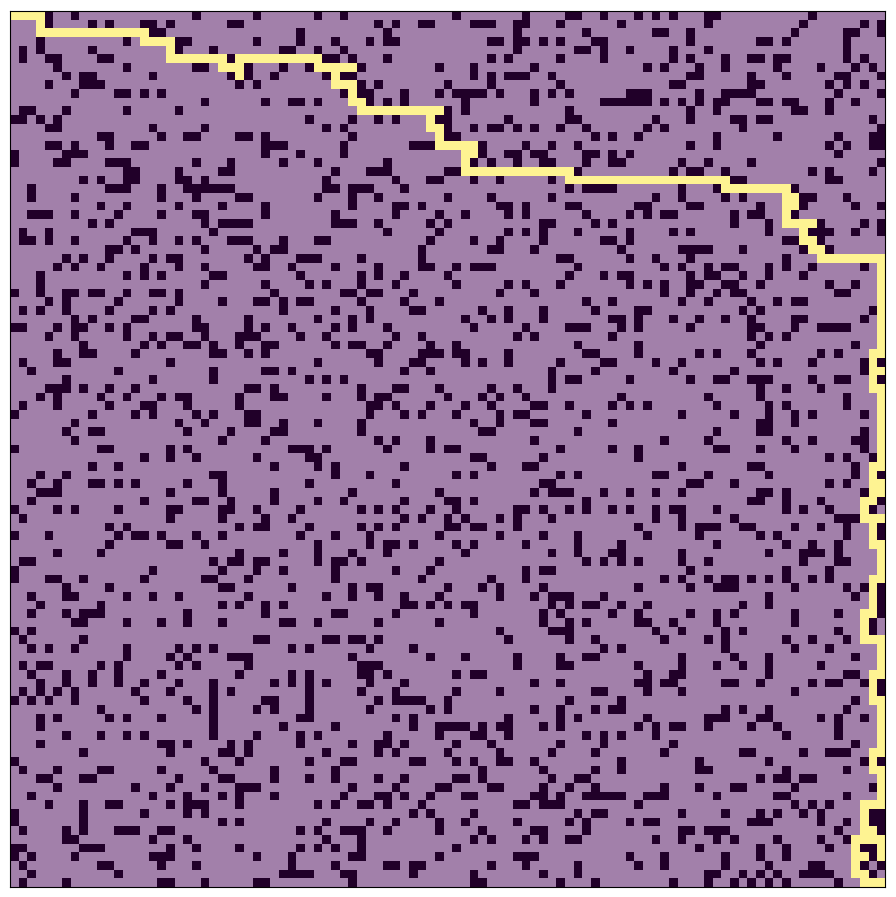
\includegraphics[width=0.8\linewidth]{Report/Part2/larger_g_forward_302.png}  
  \caption{Larger $g(n)$, 302 nodes path length}
\end{subfigure}
\begin{subfigure}{.5\textwidth}
  \centering
  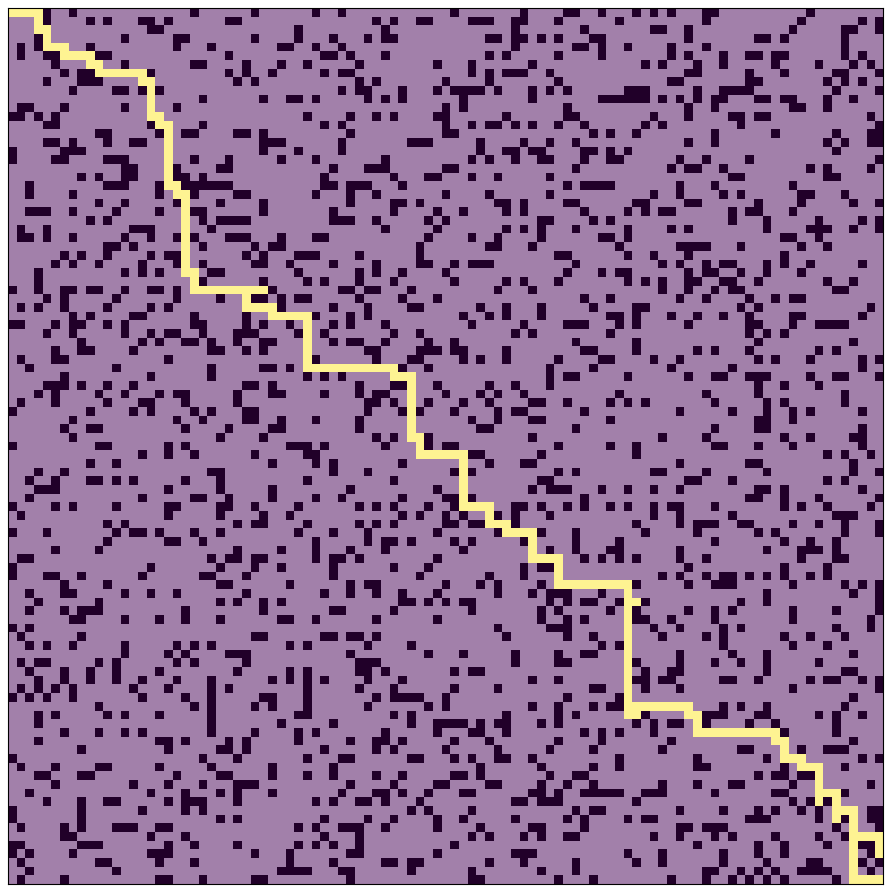
\includegraphics[width=0.8\linewidth]{Report/Part2/smaller_g_forward_260.png}  
  \caption{Smaller $g(n)$, 260 nodes path length}
\end{subfigure}
\newline
\linebreak
\linebreak
\begin{subfigure}{.5\textwidth}
  \centering
  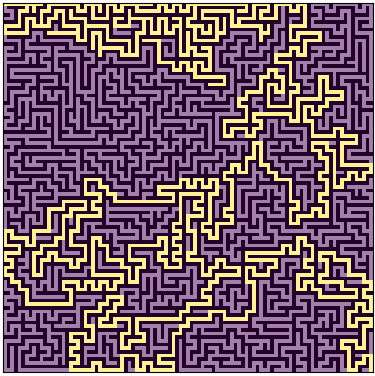
\includegraphics[width=0.8\linewidth]{Report/Part2/larger_g_forward_3178.png}  
  \caption{Larger $g(n)$, 3178 nodes path length}
\end{subfigure}
\begin{subfigure}{.5\textwidth}
  \centering
  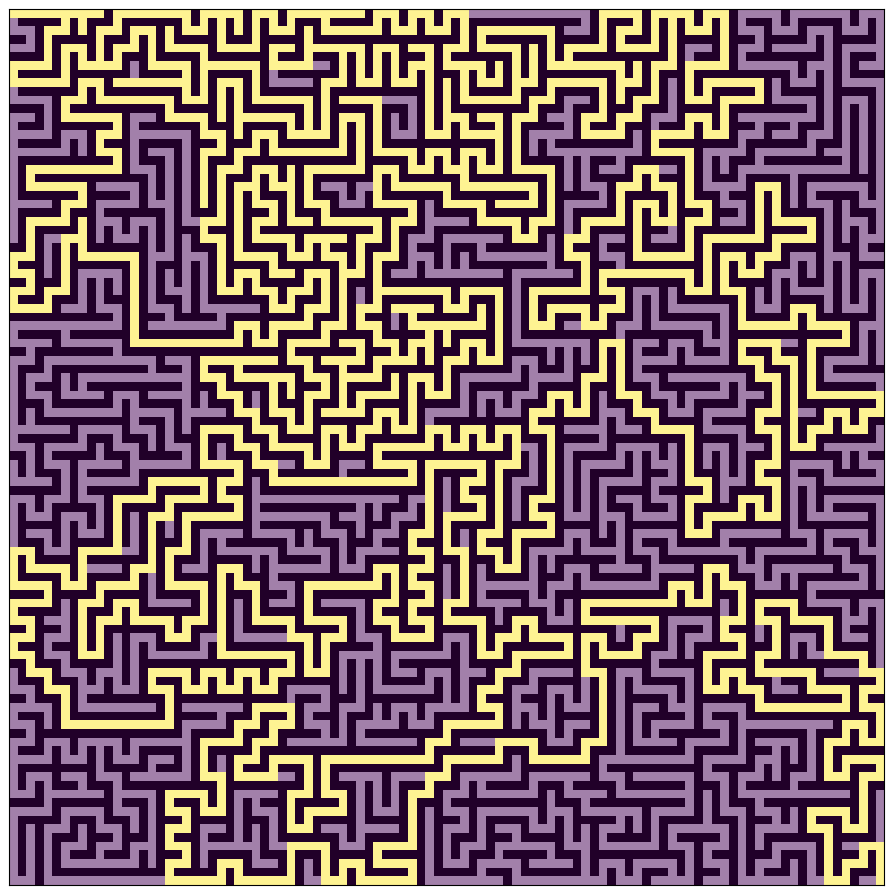
\includegraphics[width=0.8\linewidth]{Report/Part2/smaller_g_forward_4846.png}  
  \caption{Smaller $g(n)$, 4846 nodes path length}
\end{subfigure}
\caption{Repeated Forward $A^*$ tie-breaker comparison with different mazes}
\end{figure}